\subsection*{b)}

\section*{Antwort}

Es empfiehlt sich, eine \textbf{Kompositionsbeziehung} (\cite[49]{Bal05}) zu modellieren: Abbildung~\ref{fig:aufgabe-4-teil-b} zeigt einen Entwurf für eine Umsetzung in Java.\\

\begin{figure}
    \centering
    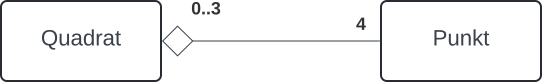
\includegraphics[scale=0.35]{chapters/aufgabe 4/img/aufgabe4b}
    \caption{Modellierung eines Quadrats als Komposition der Klassen \textit{Quadrat} und \textit{Punkt} in Java. Punkt realisiert \textit{Cloneable} und überschreibt \textit{clone()}, damit Kopien erzeugt werden können. (Quelle: eigene)}
    \label{fig:aufgabe-4-teil-b}
\end{figure}

\noindent
Die Klasse \code{Quadrat} hat als Eigenschaft 4 Objekte des Typs \code{Punkt}.\\
Die Klasse als \textit{Ganzes} übernimmt die Erzeugung der Punkte, seiner \textit{Teile}.
    \begin{itemize}
        \item Der Konstruktor \code{Quadrat(a1: double,a2: double,b1: double,b2: double,c1: double,c2: double,d1: double,d2: double)} erzeugt aus einem Paar der insg. 8 Übergabeparameter jeweils einen \code{Punkt}
        \item Der Konstruktor \code{Quadrat(a: Punkt, b: Punkt, c: Punkt, d: Punkt)} sorgt dafür, dass Kopien der \code{Punkt}-Instanzen erzeugt werden\footnote{
            hierzu realisiert \textit{Punkt} \textit{Cloneable}, s. a. \url{https://docs.oracle.com/en/java/javase/22/docs/api/java.base/java/lang/Cloneable.html}, abgerufen 18.05.2024
        }
    \end{itemize}

\noindent
\code{Quadrat} verwaltet die Punkte und stellt sicher, dass über die Methode \code{getPunkte()} \textit{Kopien} der jeweiligen Punkte zurückgeliefert werden: Änderungen der Eigenschaften der Punkte wirken sich also nicht auf \code{Quadrat} aus - damit ist \code{Quadrat} in der Hinsicht \textbf{immutable}\footnote{
vgl. \cite[21]{LG00} und insbesondere ebenda S. 94 f.
}\\

\noindent
Ein \code{Punkt} kann nur zu einem Quadrat gehören.\\
Zwar sieht die Skizze so aus, als könnte ein Punkt auch zu max. 4 Quadraten gehören (als ``Mittelpunkt``) - allerdings würde die Änderung eines solchen Punktes dann auch direkt 4 Quadrate betreffen, die sich die betreffende Referenz auf das Objekt vom Typ \code{Punkt} teilen.\\
Die \textbf{Kompositionsbeziehung} formuliert an der Stelle - im Unterschied zu einer Aggregationsbeziehung - die Ganzes-Teile-Beziehung entsprechend schärfer, damit Probleme, wie bspw. \textbf{Aliasing-Bugs}\footnote{
\url{https://martinfowler.com/bliki/AliasingBug.html}, abgerufen 18.05.2024
}) im Betrieb vermieden werden.\\

